\newpage
\section{Auswertung}
\label{sec:Auswertung}

\subsection{Verhältnis von Schwingungs- und Schwebungsfrequenz}
Die Anzahl der Maxima in einer Einhüllenden steigt mit der Kapazität an, wie \autoref{fig:plot} zeigt.
\begin{table}
  \centering
  \caption{Tabelle der Messwerte zur Schwingungsfrequenz}
  \label{tab:tab1}
  \begin{tabular}{c c}
    \toprule
    \(C_K\) in $nF$ & Anzahl Maxima\\
    \midrule
    2.03 & 4\\
    3.00 & 5\\
    4.00 & 5\\
    5.02 & 6\\
    6.47 & 8\\
    8.00 & 11\\
    9.99 & 14\\
    \bottomrule
  \end{tabular}
\end{table}

%In \autoref{fig:plot} sieht man, die Messwerte und eine Ausgleichsgerade. 
\begin{figure}
  \centering
  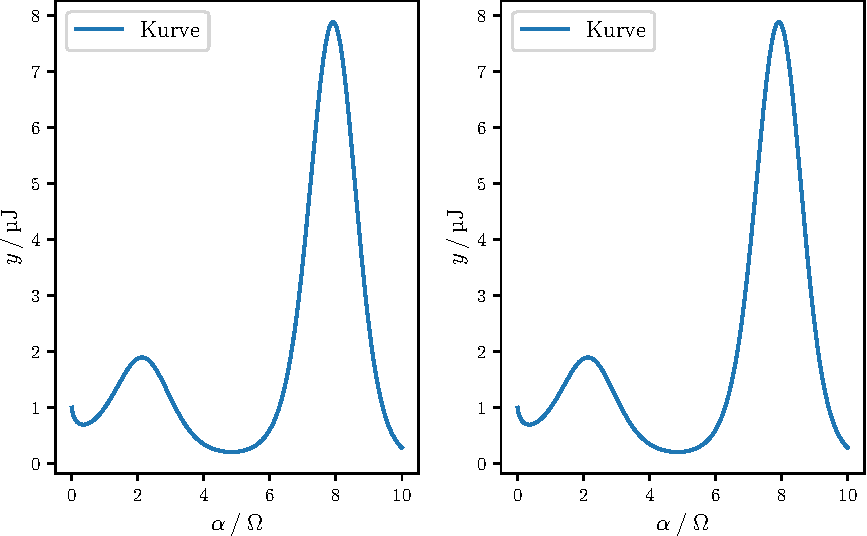
\includegraphics{plot.pdf}
  \caption{Kapazität gegen Anzahl an Maxima.}
  \label{fig:plot}
\end{figure}
Das Verhältnis muss demnach annähernd linear mit der Kapazität ansteigen.
\newpage
\subsection{Lissajou-Figuren}

\begin{table}
  \centering
  \caption{Tabelle der Messwerte zur Phasenverschiebung}
  \label{tab:tab2}
  \begin{tabular}{c c c}
    \toprule
    \(C_K\) in $nF$ & \(\nu_-\) in $Hz$ & \(\nu_+\) in $Hz$\\
    \midrule
    1.01 & 47090 & 30450\\
    2.03 & 39990 & 30440\\
    3.00 & 37275 & 30440\\
    4.00 & 35730 & 30440\\
    5.02 & 34760 & 30440\\
    6.47 & 33870 & 30440\\
    8.00 & 33260 & 30440\\
    9.99 & 32740 & 30440\\
    \bottomrule
  \end{tabular}
\end{table}

\autoref{fig:plot2} zeigt die Frequenzen, bei denen unter verschiedenen Kapazitäten die Phasenverschiebung 0 beträgt, also \(\nu_-\), oder \(\pi\), also \(\nu_+\).
Es ist sehr deutlich zu sehen, dass die Phasenverschiebung um \(\pi\) so gut wie immer bei der selben Frequenz erfolgt, unabhängig von der Kapazität.
\(\nu_-\) hingegen fällt mit zunehmender Kapazität exponentiell ab.
\begin{figure}
  \centering
  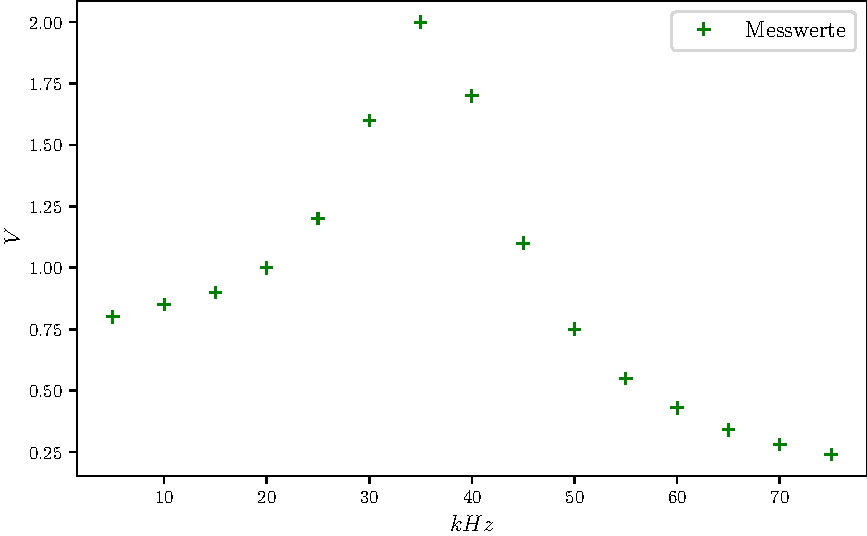
\includegraphics{plot2.pdf}
  \caption{Kapazität gegen Frequenz.}
  \label{fig:plot2}
\end{figure}
\newpage
\subsection{Stromverlauf im gekoppeltem Schwingkreis}

\begin{table}
  \centering
  \caption{Tabelle der Messwerte zur Phasenverschiebung}
  \label{tab:tab2}
  \begin{tabular}{c c c c c}
    \toprule
    \(C_K\) in $nF$ & Erste Ampl & Zweite Ampl & a in $ms$ & b in $ms$\\
    \midrule
    2.03 & 1.75 & 1.4 & 17.5 & 29.5\\
    3.00 & 1.75 & 1.5 & 18 & 21.5\\
    4.00 & 1.75 & 1.55 & 18 & 16.5\\
    5.02 & 1.75 & 1.55 & 17.5 & 13.5\\
    6.47 & 1.75 & 1.6 & 17.5 & 10.5\\
    8.00 & 1.8 & 1.6 & 17.5 & 8.5\\
    9.99 & 1.8 & 1.6 & 18 & 6.5\\
    \bottomrule
  \end{tabular}
\end{table}

Die \autoref{fig:plot3} zeigt die jeweiligen Amplituden der Kurve des Oszilloskops und ihre Entfernung zueinander in ms.
Die zweite Amplitude befindet sich genau \(s = a + b\) von \(t = 0\).
Je näher die zweite Amplitude ist, desto höher ist die Kapazität \(C_K\).
Man kann annehmen, dass sich die Position der ersten Amplitude so gut wie nicht verändert.
\begin{figure}
  \centering
  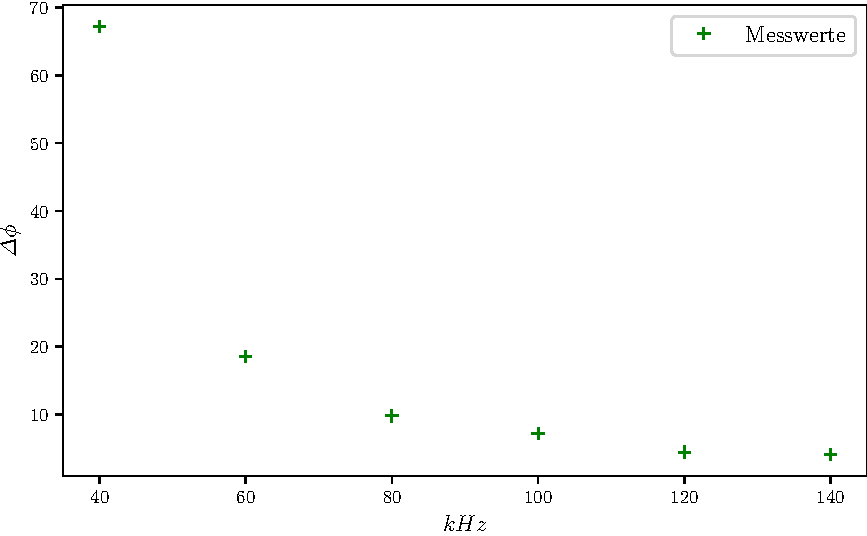
\includegraphics{plot3.pdf}
  \caption{Spannung gegen Zeit.}
  \label{fig:plot3}
\end{figure}